
\section{Empirical Confirmation}
\label{sec:emp}

Our convergence results hold exactly in relation to $M$ (and $N$) but are only 
asymptotic in $K$ due to the higher order terms.  Therefore their applicability should be viewed with a 
healthy degree of skepticism in the small $K$ regime.
 With this in mind, we now present empirical support for our theoretical results 
and test how well they hold in the small $K$ regime
 using a simple Gaussian model, for which we can analytically calculate the ground truth.
 
 Consider a family of generative models with $\mathbb R^D$--valued latent variables $z$ and observed variables $x$:
\begin{align}
    z \sim \mathcal{N}(z;\mu, I), &&
    x \given z \sim \mathcal{N}(x; z, I),
\end{align}
which is parameterized by $\theta := \mu$.
Let the inference network be parameterized by $\phi = (A, b), \; A \in \mathbb R^{D \times D}, \; b \in \mathbb R^D$ where $q_{\phi}(z \given x) = \mathcal{N}(z; Ax + b, \frac{2}{3}I )$.
Given a dataset $(x^{(n)})_{n = 1}^N$, we can analytically calculate the optimum of our target $\mathcal J(\theta, \phi)$ as explained in Appendix~\ref{sec:optGauss},
giving $\theta^* := \mu^* = \frac{1}{N} \sum_{n = 1}^N x^{(n)}$ and 
$\phi^* := (A^*, b^*)$, where $A^* = I / 2$ and $b^* = \mu^* / 2$. Though this will not be the
case in general, for
this particular problem, the optimal proposal is independent of $K$. 
However, the expected gradients for the inference network still change with $K$.


\begin{figure*}[t]
	\centering
	\begin{subfigure}[b]{0.4\textwidth}
		\centering
		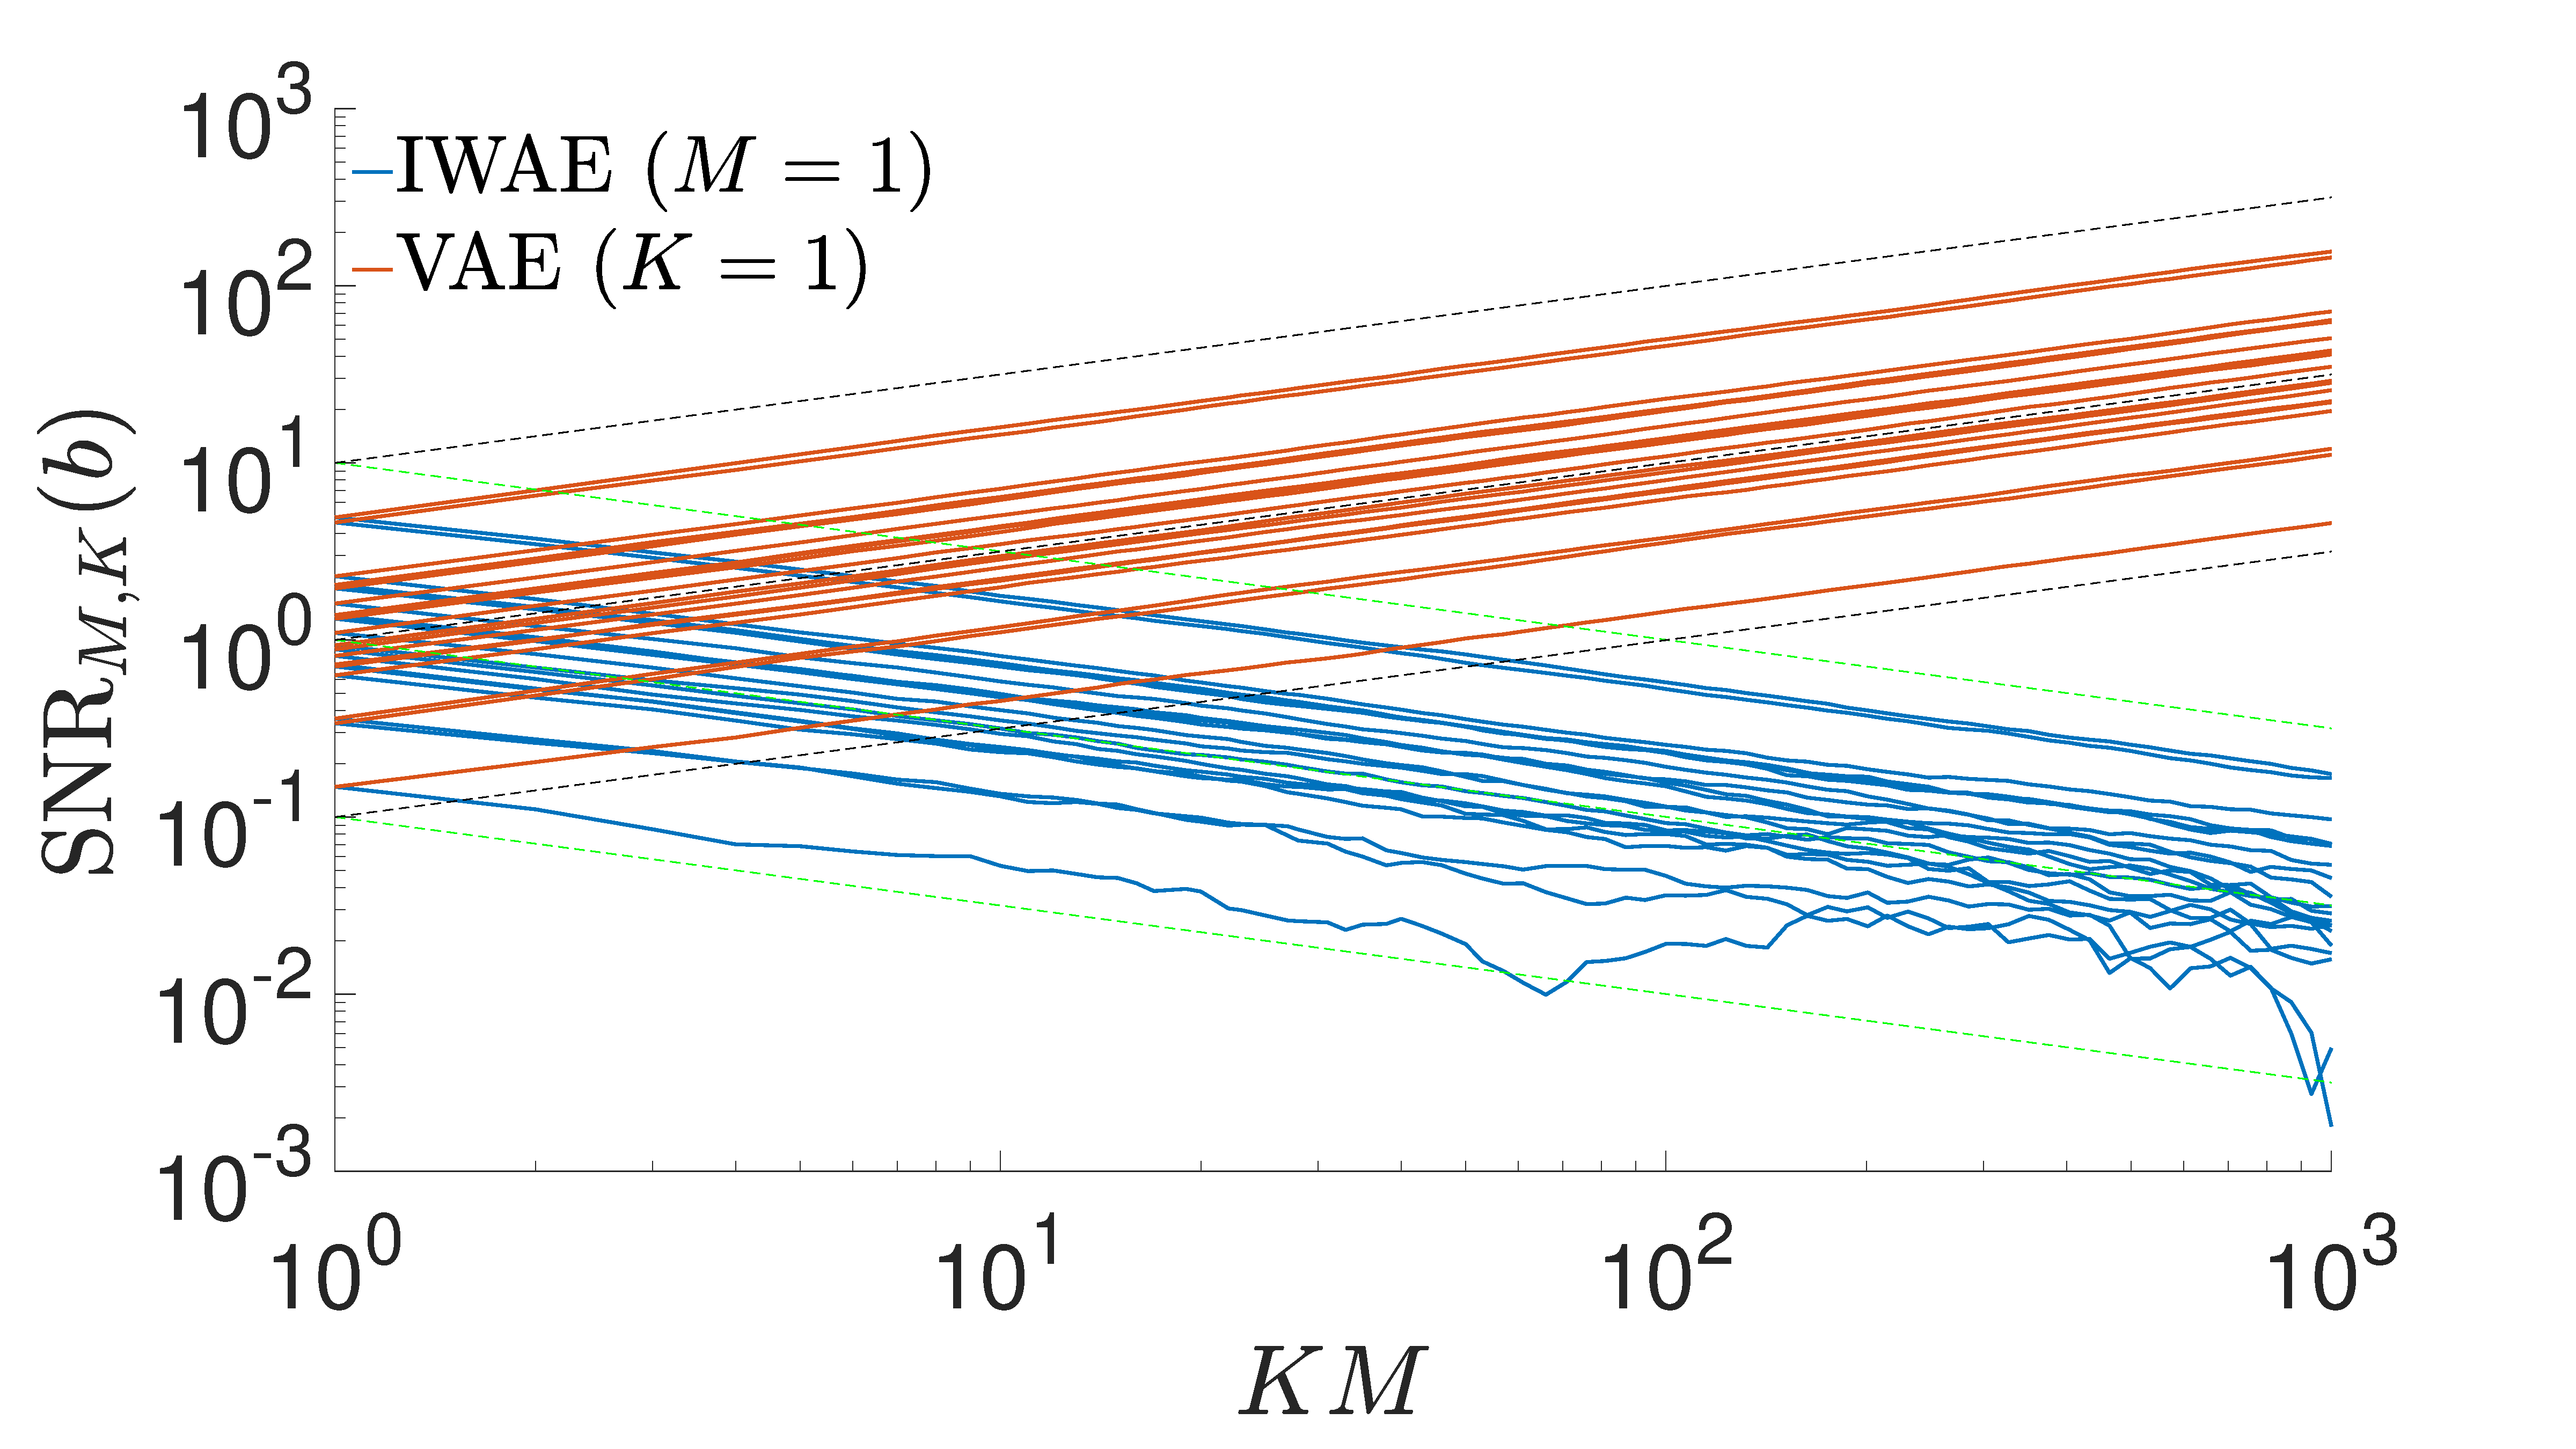
\includegraphics[width=\textwidth]{figures/tighter_bounds/b_conv}
		\caption{Convergence of \gls{SNR} for inference network \label{fig:snr/b}}
	\end{subfigure}
	\begin{subfigure}[b]{0.4\textwidth}
		\centering
		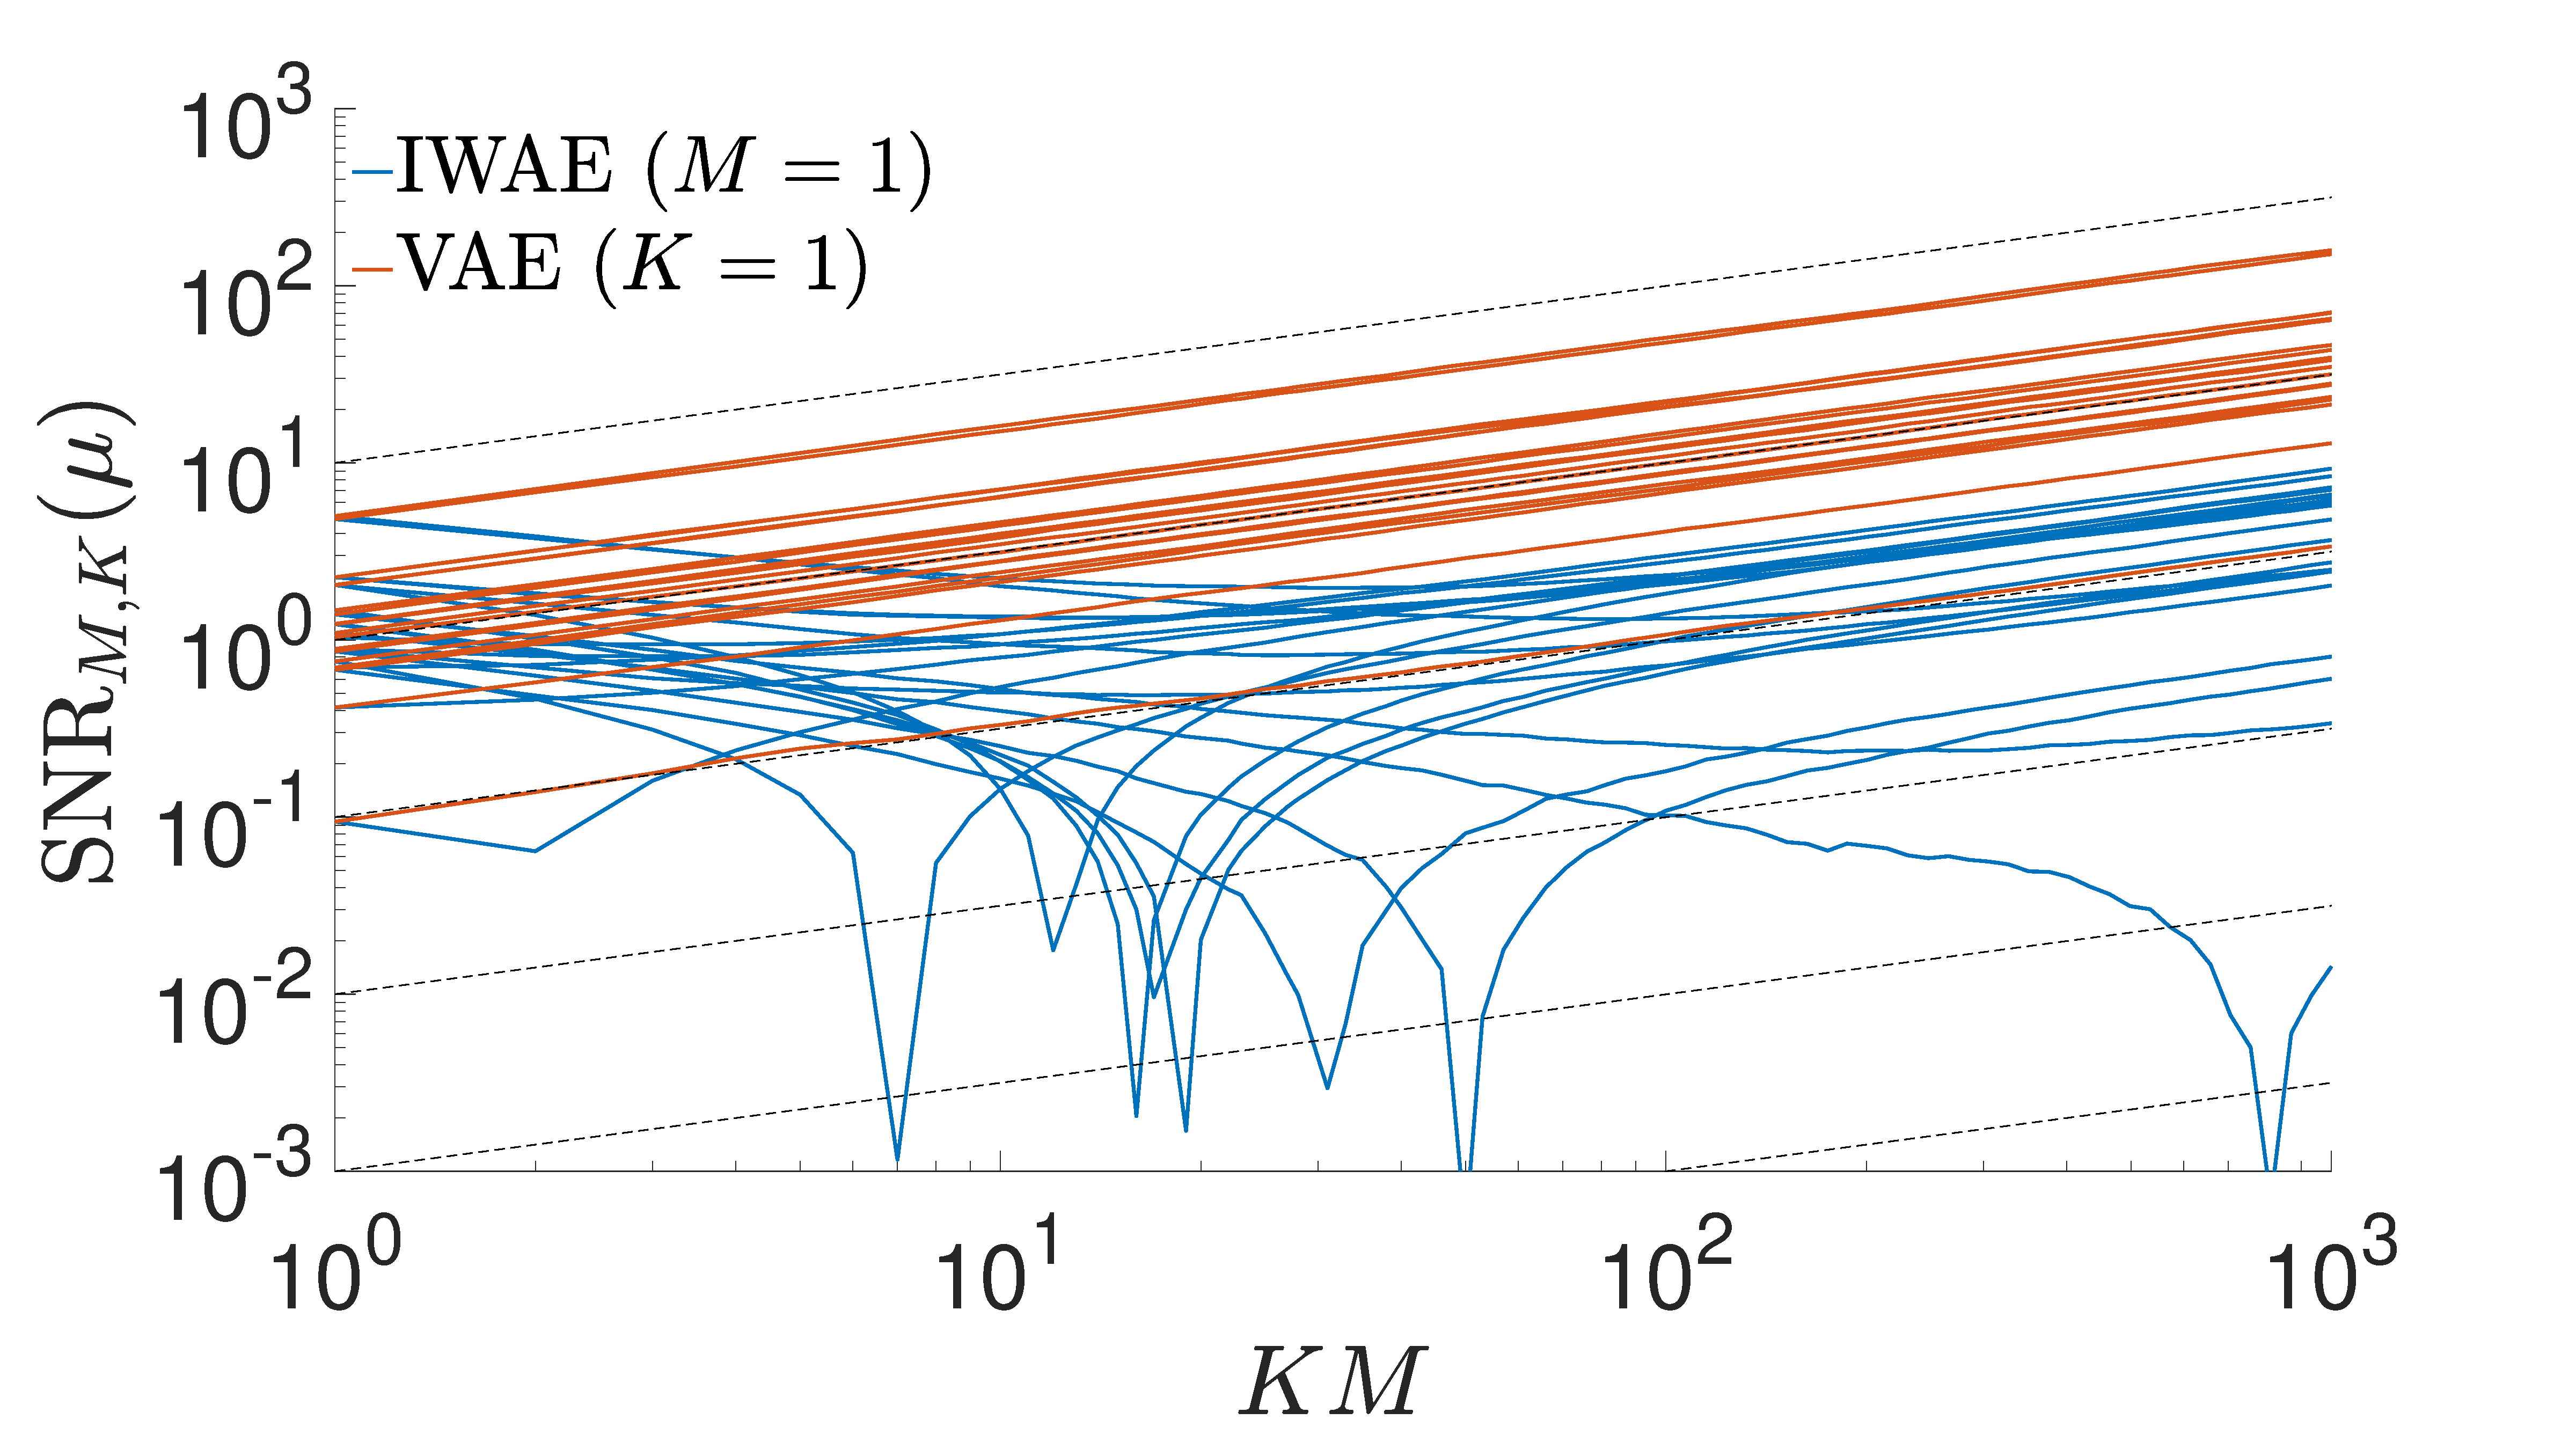
\includegraphics[width=\textwidth]{figures/tighter_bounds/mu_conv}
		\caption{Convergence of \gls{SNR} for generative network\label{fig:snr/mu}}
	\end{subfigure}
	\caption{Convergence of signal-to-noise ratios of gradient estimates with increasing $M$ and $K$.
		Different lines correspond to different
		dimensions of the parameter vectors.
		Shown in blue is the \gls{IWAE} where we keep $M=1$ fixed and increase $K$.  
		Shown in red is the \gls{VAE} where $K=1$ is fixed and we increase $M$. 
		The black and green dashed lines show the expected convergence rates from our theoretical results, 
		representing gradients of $1/2$ and $-1/2$ respectively.  
		\label{fig:snr/K_conv}}
\end{figure*}

To conduct our investigation, we randomly generated a synthetic dataset from the model with $D=20$
dimensions, $N=1024$ data points, and a true model parameter value $\mu_{\text{true}}$ that was itself 
randomly generated from a unit Gaussian, i.e. $\mu_{\text{true}} \sim \mathcal{N}(\mu_{\text{true}} ;0,I)$.
We then considered the gradient at a random point in the parameter space close to optimum (we also 
	consider a point far from the optimum in 
	Appendix~\ref{sec:hv}). Namely
each dimension of each parameter was randomly offset from its optimum value using a zero-mean
Gaussian with standard deviation $0.01$.  We then calculated empirical estimates of the \gls{ELBO}
gradients for \gls{IWAE}, where $M=1$ is held fixed and we increase $K$, and
for \gls{VAE}, where $K=1$ is held fixed and we increase $M$.  In all cases we 
calculated $10^4$ such estimates and used these samples to provide empirical estimates for, amongst other things, the
mean and standard deviation of the estimator, and thereby an empirical estimate for the \gls{SNR}.

We start by examining the qualitative behavior of the different gradient estimators as $K$ increases as
shown in Figure~\ref{fig:snr/hists}.  This shows histograms of the \gls{IWAE}  gradient estimators
for a single parameter of the inference network (left) and generative network (right).
We first see in Figure~\ref{fig:snr/b_hist_iwae} that as $K$ increases, both the magnitude and the standard
deviation of the estimator decrease for the inference network, 
with the former decreasing faster.  This
matches the qualitative behavior of our theoretical result, with the \gls{SNR} ratio 
diminishing as $K$ increases.
In particular, the probability that the gradient is positive or negative 
becomes roughly equal for larger
values of $K$, meaning the optimizer is equally likely to increase as decrease the 
inference network parameters at the next iteration.
By contrast, for the generative network, \gls{IWAE} converges towards a 
non-zero gradient, such that,
even though the \gls{SNR} initially decreases with $K$, it then rises again, with a very
clear gradient signal for $K=1000$.


To provide a more rigorous analysis, we next directly examine the convergence of 
the \gls{SNR}.
Figure~\ref{fig:snr/K_conv} shows the convergence of the estimators with increasing $M$ and $K$.
The observed rates for the inference network (Figure~\ref{fig:snr/b})
correspond to our theoretical results, with
the suggested rates observed all the way back to $K=M=1$.  As expected, we see 
that as $M$ increases, so does $\SNR_{M,K}(b)$, but as $K$ increases, $\SNR_{M,K}(b)$ reduces.

In Figure~\ref{fig:snr/mu}, we see that
the theoretical convergence for $\SNR_{M,K}(\mu)$
is again observed exactly for variations in $M$, 
but a more unusual behavior is seen for variations in $K$,
where the \gls{SNR} initially decreases before starting to increase again for large enough $K$, 
eventually exhibiting behavior consistent with the theoretical result for large enough $K$.
The driving factor for this is that here
$\E [\Delta_{M,\infty}(\mu)]$  has a smaller magnitude than (and opposite sign to)
$\E [\Delta_{M,1}(\mu)]$  (see Figure~\ref{fig:snr/mu_hist_iwae}).  If we think of the estimators
for all values of $K$ as biased estimates for
$\E [\Delta_{M,\infty}(\mu)]$, we see from our theoretical results that this bias decreases faster 
than the standard deviation.  Consequently, while the magnitude of this bias remains large compared to
$\E [\Delta_{M,\infty}(\mu)]$, it is the predominant component in the true gradient and
we see similar \gls{SNR} behavior as in the inference network.

Note that this does not mean that the 
estimates are getting worse for the generative network.
As we increase $K$ our bound is getting tighter and our estimates closer to
the true gradient for the target that we 
actually want to optimize $\nabla_{\mu} \log Z$.  See 
Appendix~\ref{sec:app:rmse} for more details.
As we previously discussed, it is also the case that increasing $K$ could be beneficial for the inference network
even if it reduces the \gls{SNR} by improving the direction of the expected gradient.
However, as we will now show, the \gls{SNR} is, for this problem,
the dominant effect for the inference network.

\begin{figure*}[t]
	\centering
	\begin{subfigure}[b]{0.4\textwidth}
		\centering
		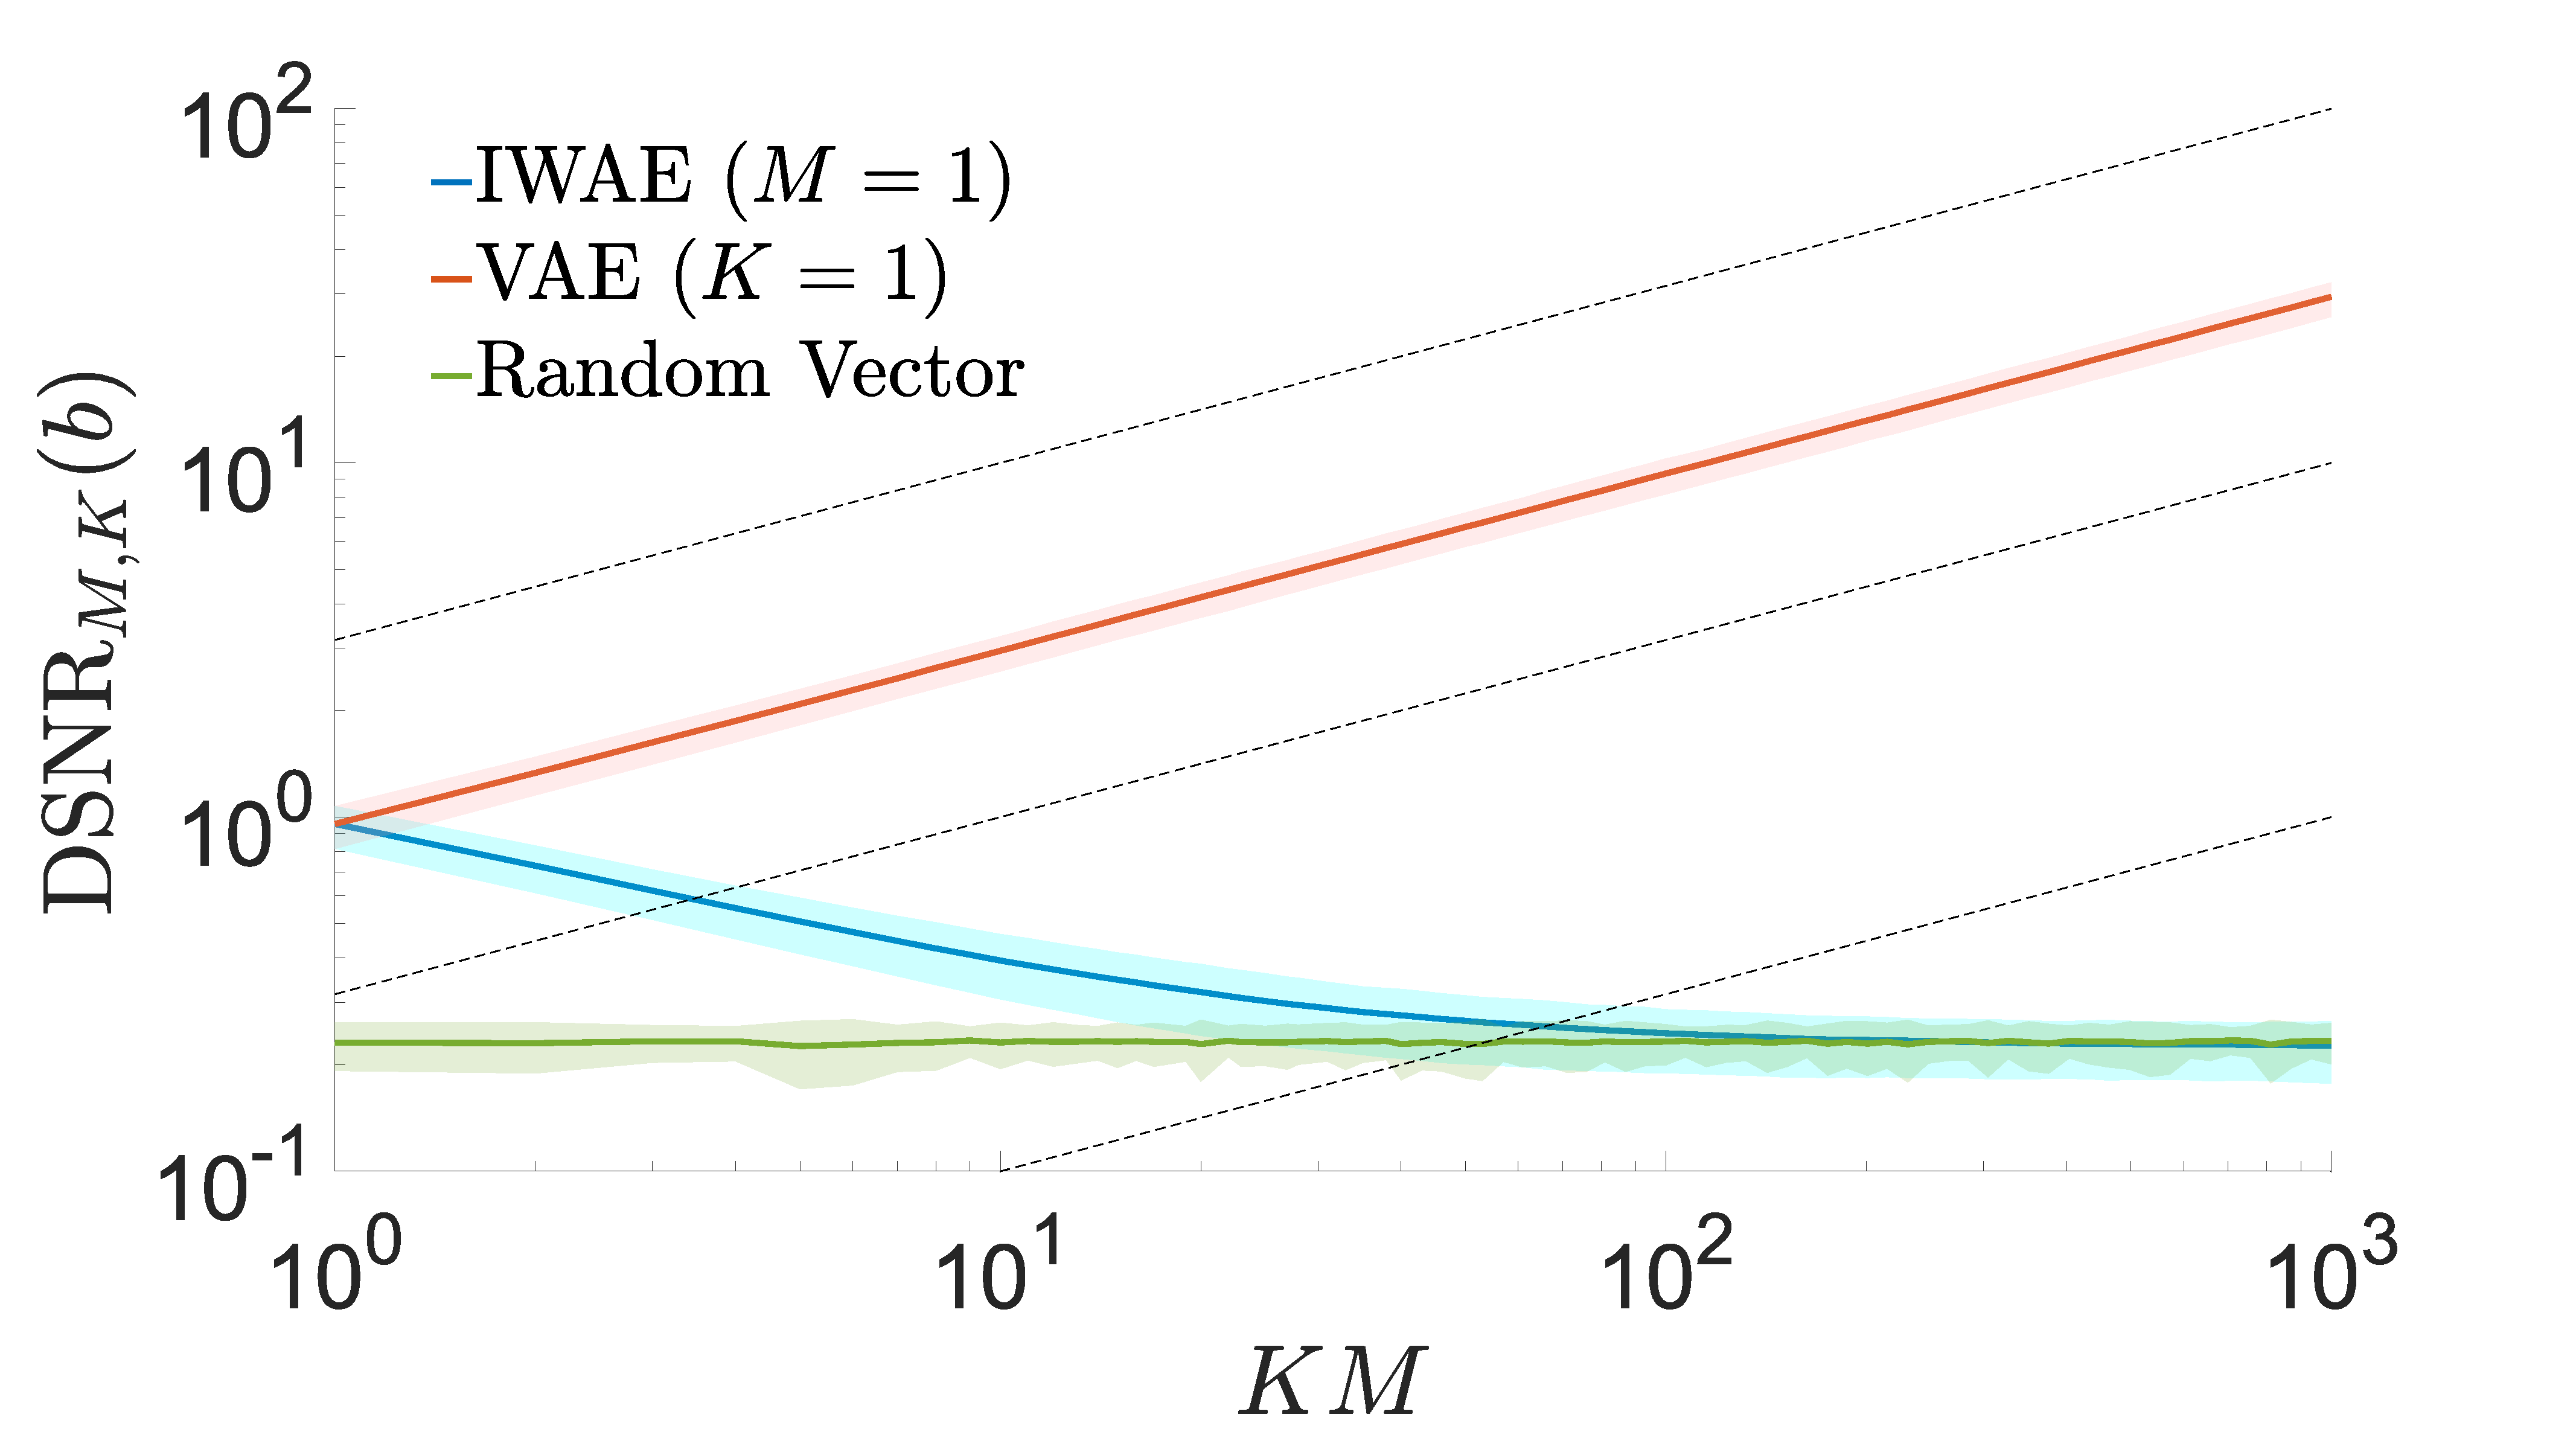
\includegraphics[width=\textwidth]{figures/tighter_bounds/snr_dir}
		\caption{Convergence of \textsc{dsnr} for inference network\label{fig:snr/snr_dir}}
	\end{subfigure}
~~~~~~~~~~~~~~
	\begin{subfigure}[b]{0.4\textwidth}
		\centering
		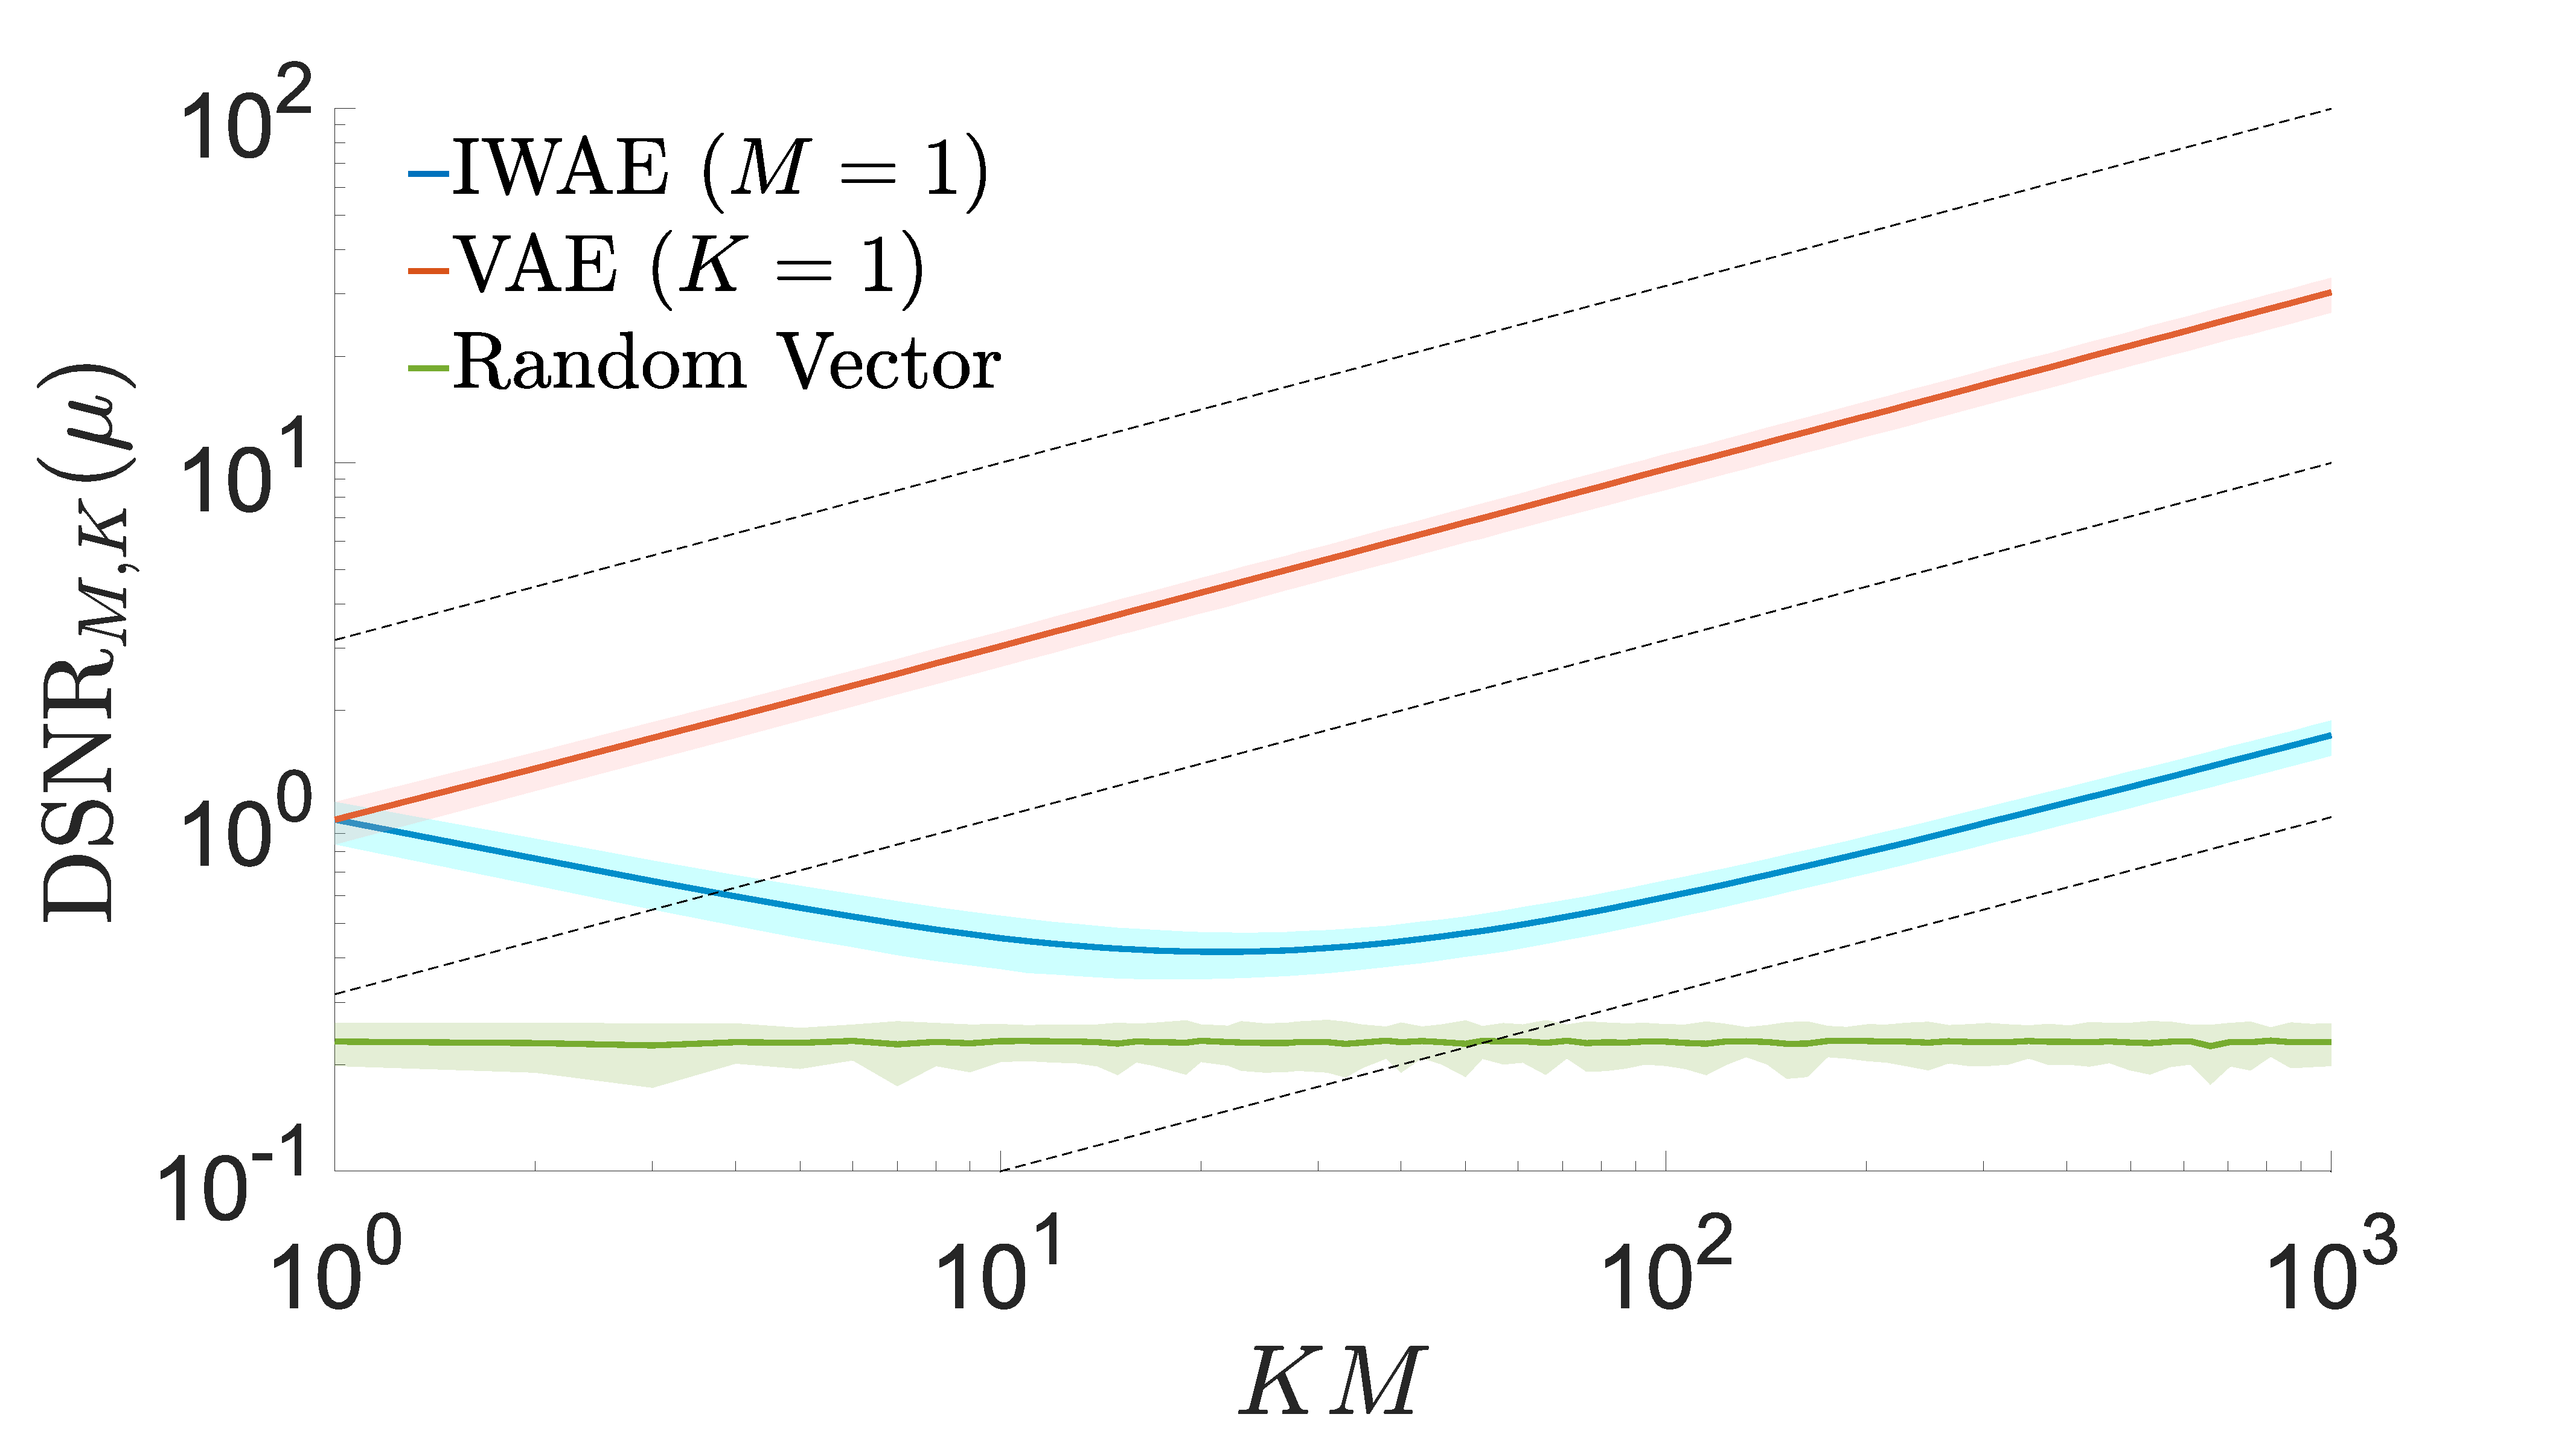
\includegraphics[width=\textwidth]{figures/tighter_bounds/snr_dir_mu}
		\caption{Convergence of \textsc{dsnr} for generative network\label{fig:snr/snr_dir_mu}}
	\end{subfigure}\vspace{-6pt}
	\caption{Convergence of the directional \gls{SNR} of gradients estimates with increasing $M$ and $K$.
		The solid lines show the estimated \textsc{dsnr} and the shaded regions the interquartile range of
		the individual ratios.  Also shown for reference is the \textsc{dsnr} for a randomly generated
		vector where each component is drawn from a unit Gaussian.
		\vspace{-10pt}
		\label{fig:snr/extra}}
\end{figure*}

\begin{figure*}[t]
	\centering
	\begin{subfigure}[b]{0.4\textwidth}
		\centering
		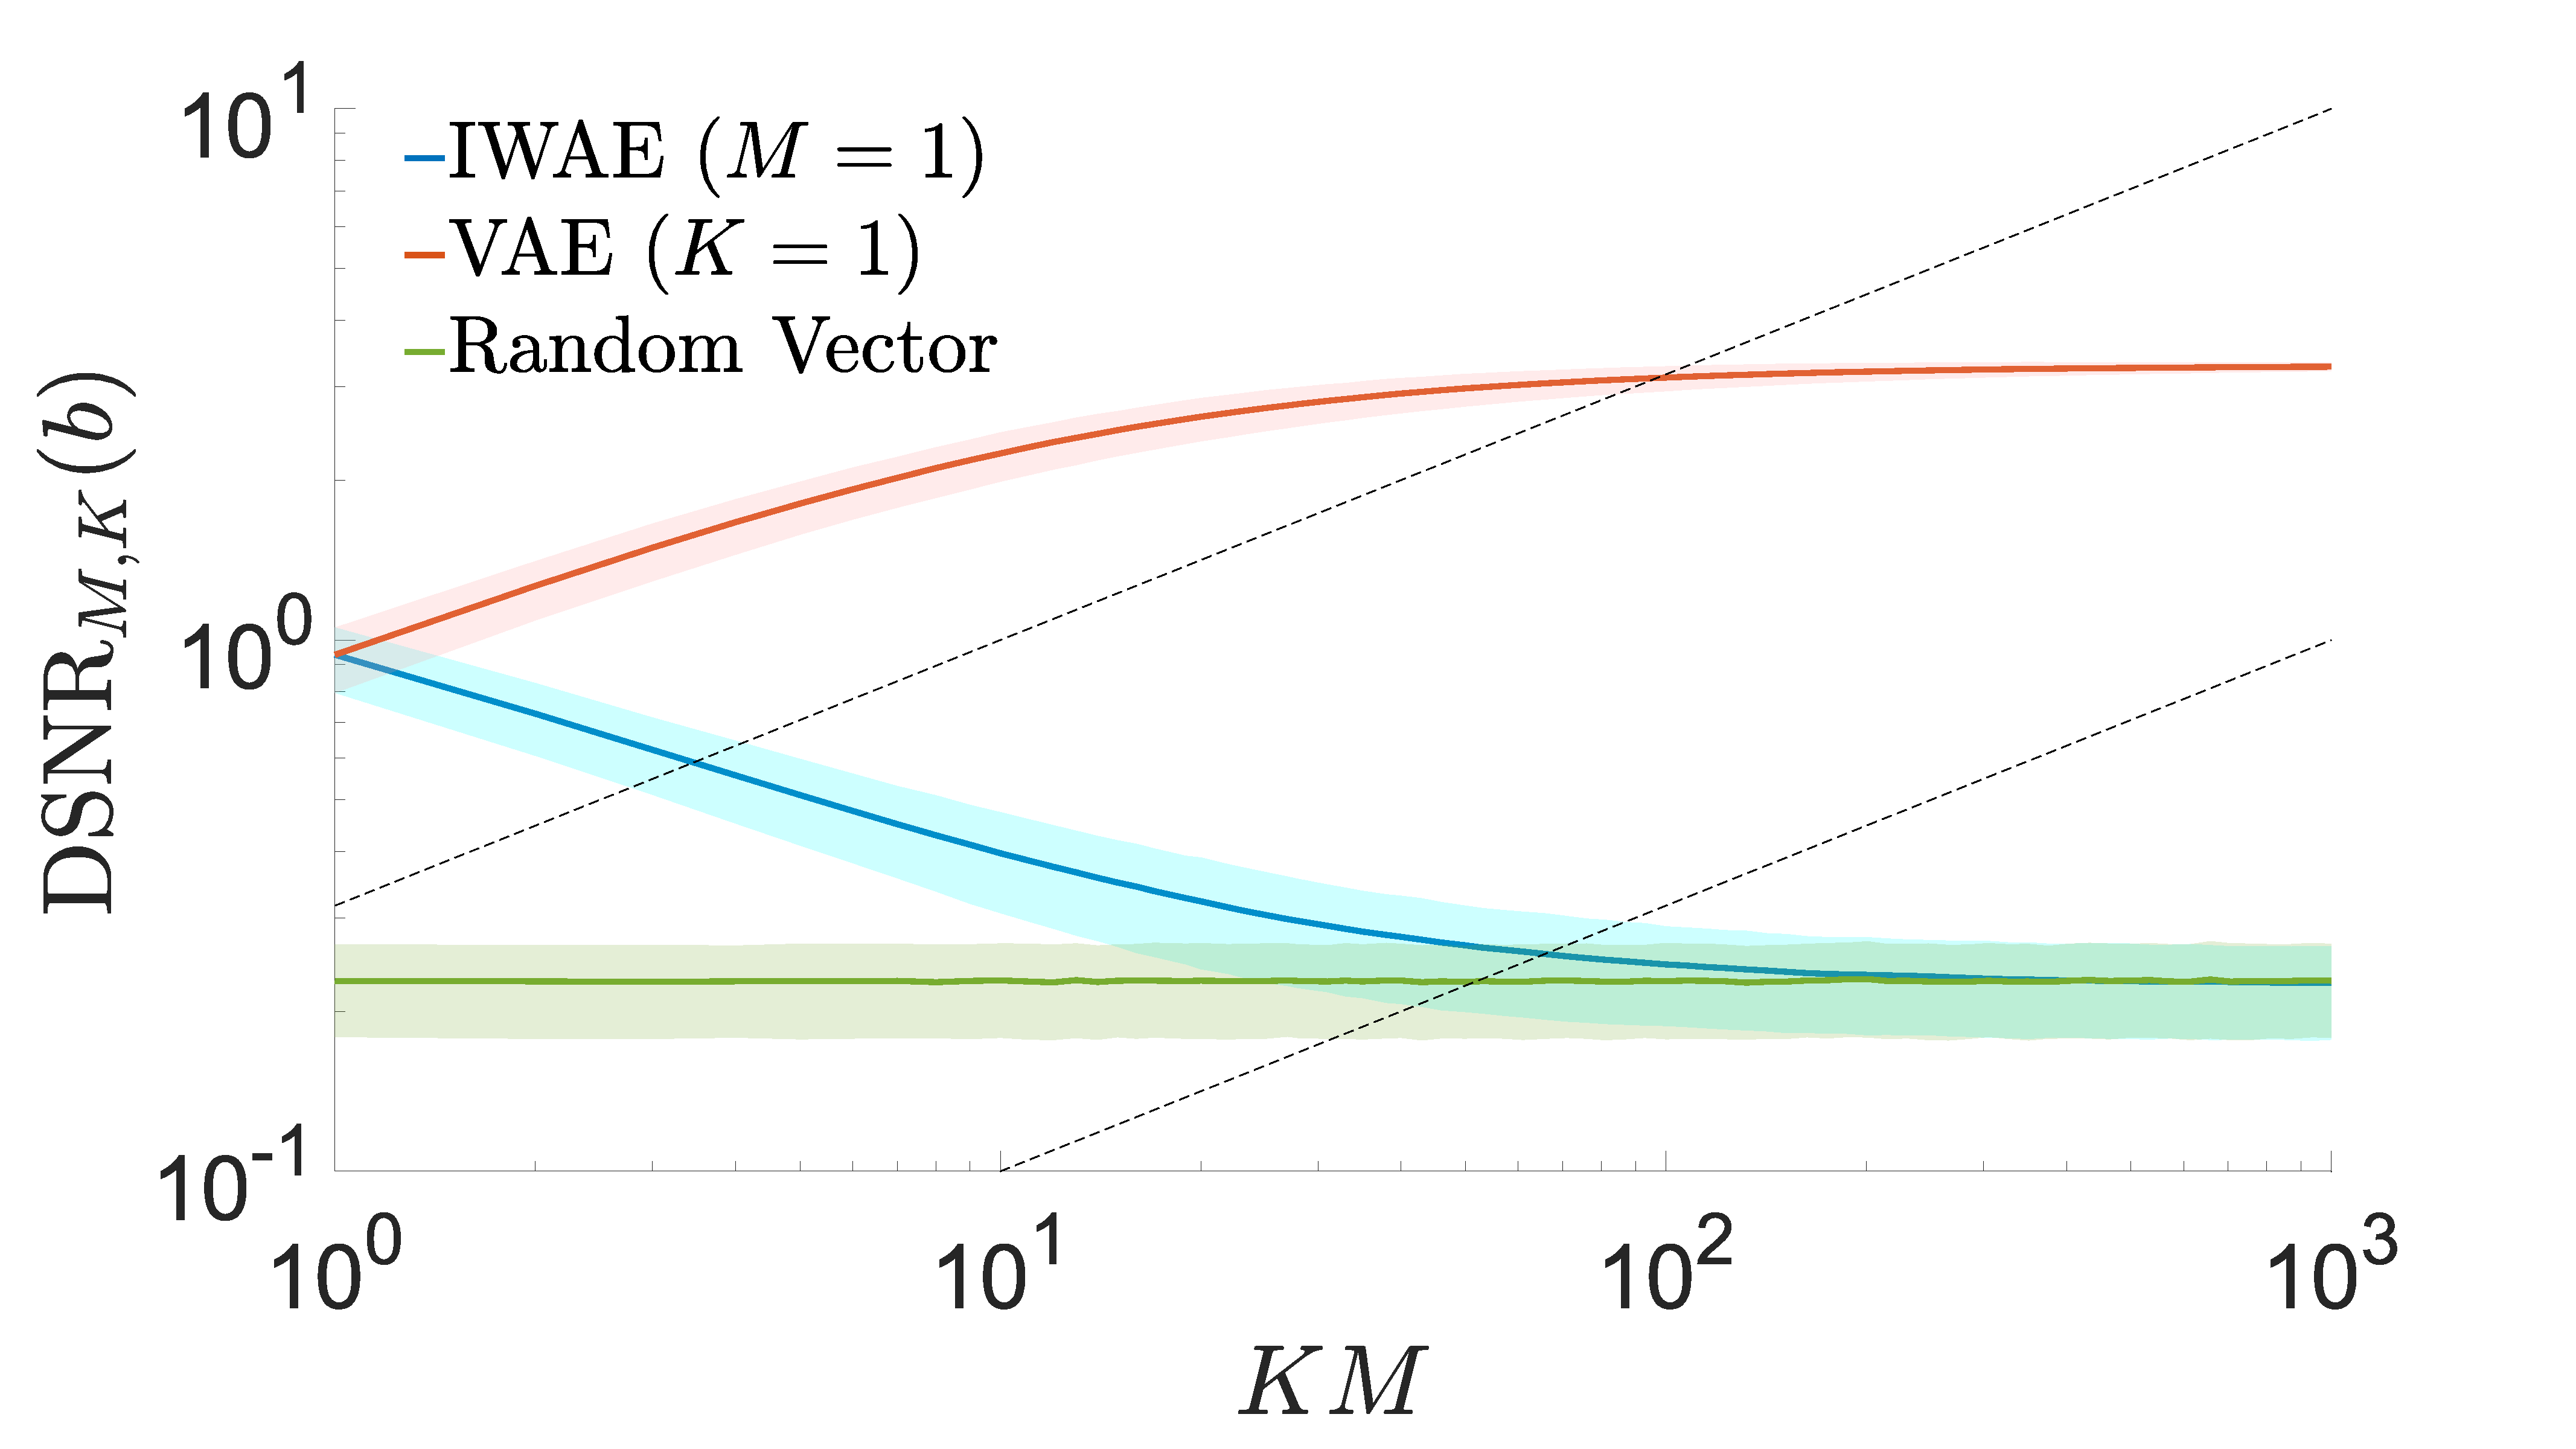
\includegraphics[width=\textwidth]{figures/tighter_bounds/dir_snr_end}
		\caption{Convergence of \textsc{dsnr} for inference network\label{fig:snr/snr_dir_end}}
	\end{subfigure} ~~~~~~~~~~~~~~
	\begin{subfigure}[b]{0.4\textwidth}
		\centering
		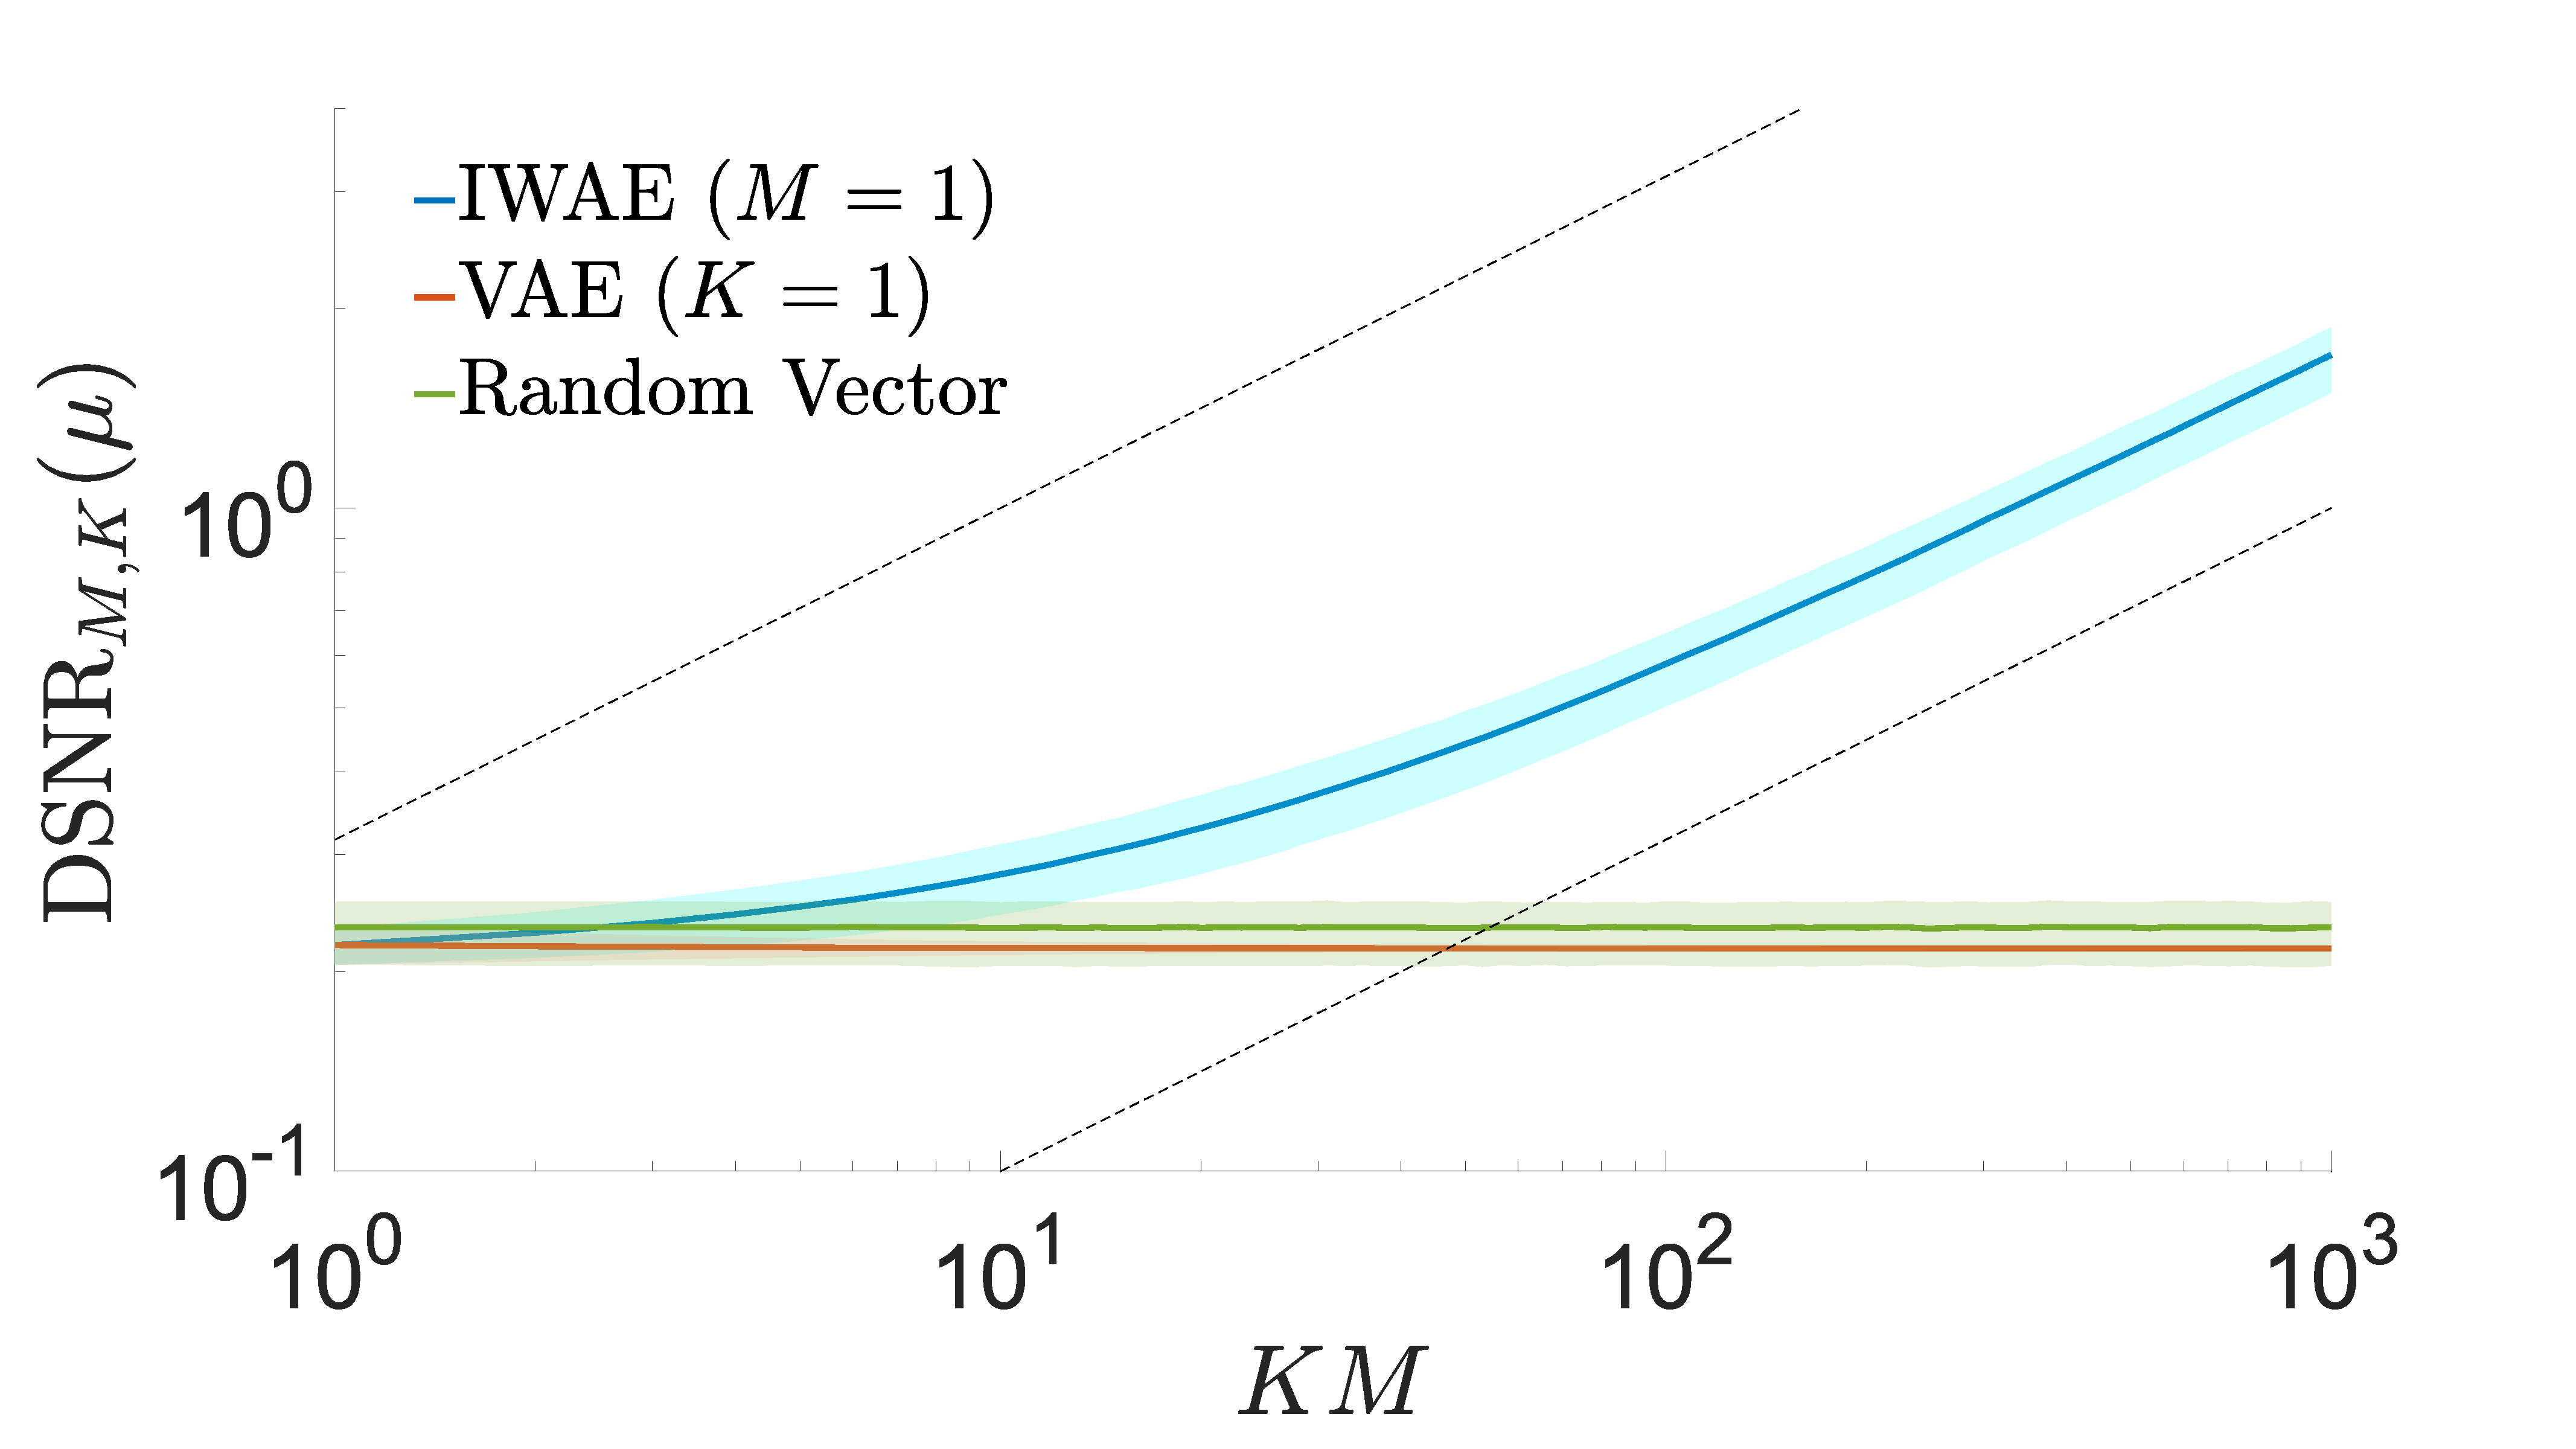
\includegraphics[width=\textwidth]{figures/tighter_bounds/dir_snr_mu_end}
		\caption{Convergence of \textsc{dsnr} for generative network\label{fig:snr/snr_dir_mu_end}}
	\end{subfigure}
	\caption{Convergence of the \textsc{dsnr} when the
		target gradient is taken as $u = \E \left[\Delta_{1,1000}\right]$.  Conventions as
		per Figure~\ref{fig:snr/extra}.
		\label{fig:snr/extra_end}}
\end{figure*}


\subsection{Directional Signal-to-Noise Ratio}

As a reassurance that our chosen definition of the \gls{SNR} is appropriate
for the problem at hand and to examine the effect of multiple dimensions explicitly,
 we now also consider an alternative definition of the \gls{SNR} that is similar (though distinct)
to that used in~\cite{Roberts2009signal}.  We refer to this as the ``directional'' \gls{SNR} (\textsc{dsnr}).
At a high-level, we define the \textsc{dsnr} by splitting each gradient estimate into two component vectors, one parallel
to the true gradient and one perpendicular, then taking the expectation of ratio of their magnitudes.  More precisely,
we define $u =\E \left[\Delta_{M,K}\right]/\lVert\E \left[\Delta_{M,K}\right]\rVert_2$ as being
the true normalized gradient direction and then the \textsc{dsnr} as
\begin{align}
\textsc{dsnr}_{M,K} = & \,\,\E \left[\frac{\lVert\Delta_{\|}\rVert_2}{\lVert\Delta_{\bot}\rVert_2} \right]
\quad \text{where}  \displaybreak[0]\\
\Delta_{\|} = \left(\Delta_{M,K}^T u\right)u &\quad \text{and} \quad
\Delta_{\bot} = \Delta_{M,K}- \Delta_{\|}. \nonumber
\end{align}
The \textsc{dsnr} thus provides a measure of the expected proportion of the gradient that will point in the
true direction.  For perfect estimates of the gradients, then $\textsc{dsnr}\to\infty$, but unlike the
\gls{SNR}, arbitrarily bad estimates do not have $\textsc{dsnr}=0$ because even random vectors will have
a component of their gradient in the true direction.

The convergence of the \textsc{dsnr} is shown in Figure~\ref{fig:snr/extra}, for which the true normalized
gradient $u$ has been estimated empirically, noting that this varies with $K$.
We see a similar qualitative behavior
to the \gls{SNR}, with the gradients of \gls{IWAE} for the inference network degrading to having the
same directional accuracy as drawing a random vector.  Interestingly, the \textsc{dsnr} seems to be
following the same asymptotic convergence behavior as the \gls{SNR} for both
networks in $M$ (as shown by the dashed lines), even though we have no theoretical result to suggest this should occur.



As our theoretical results suggest that the direction of the true gradients correspond to
targeting an improved objective 
as $K$ increases, we now examine whether this or the changes in
the \gls{SNR} is the dominant effect.  To this end, we repeat our calculations for
the \textsc{dsnr} but take $u$ as the target direction of the gradient for $K=1000$. 
This provides a measure of how varying $M$ and $K$ affects the quality of the gradient directions
as biased estimators for $\E\left[\Delta_{1,1000}\right]
/\lVert\E\left[\Delta_{1,1000}\right]\rVert_2$.  As shown in Figure~\ref{fig:snr/extra_end}, increasing $K$ is still detrimental for the inference network
by this metric, even though
it brings the expected gradient estimate closer to the target gradient.  By contrast, increasing
$K$ is now monotonically beneficial for the generative network.  Increasing $M$
leads to initial improvements for the inference network before plateauing due to the bias 
of the estimator.  For the generative network, increasing $M$ has little impact, with the bias being
the dominant factor throughout.  Though this metric is not an absolute measure of
performance of the~\gls{SGA} scheme, e.g. because high bias may be more detrimental than high variance,
it is nonetheless a powerful result in suggesting that increasing $K$ can be detrimental
to learning the inference network.


